\documentclass[10pt, landscape]{article}
\usepackage[scaled=0.92]{helvet}
\usepackage{calc}
\usepackage{multicol}
\usepackage[a4paper,margin=3mm,landscape]{geometry}
\usepackage{amsmath,amsthm,amsfonts,amssymb}
\usepackage{color,graphicx,overpic}
\usepackage{hyperref}
\usepackage{newtxtext} 
\usepackage{enumitem}
\usepackage[table]{xcolor}
\usepackage{mathtools}
\setlist{nosep}
% for including images
\graphicspath{ {./images/} }

\pdfinfo{
  /Title (CS3230.pdf)
  /Creator (TeX)
  /Producer (pdfTeX 1.40.0)
  /Author (Jovyn Tan)
  /Subject (CS3230)
/Keywords (CS3230, nus,cheatsheet,pdf)}

% Turn off header and footer
\pagestyle{empty}

% redefine section commands to use less space
\makeatletter
\renewcommand{\section}{\@startsection{section}{1}{0mm}%
  {-1ex plus -.5ex minus -.2ex}%
  {0.5ex plus .2ex}%x
{\normalfont\large\bfseries}}
\renewcommand{\subsection}{\@startsection{subsection}{2}{0mm}%
  {-1explus -.5ex minus -.2ex}%
  {0.5ex plus .2ex}%
{\normalfont\normalsize\bfseries}}
\renewcommand{\subsubsection}{\@startsection{subsubsection}{3}{0mm}%
  {-1ex plus -.5ex minus -.2ex}%
  {1ex plus .2ex}%
{\normalfont\small\bfseries}}%
\makeatother

\renewcommand{\familydefault}{\sfdefault}
\renewcommand\rmdefault{\sfdefault}
%  makes nested numbering (e.g. 1.1.1, 1.1.2, etc)
\renewcommand{\labelenumii}{\theenumii}
\renewcommand{\theenumii}{\theenumi.\arabic{enumii}.}
\renewcommand\labelitemii{•}
\renewcommand\labelitemiii{•}

\definecolor{mathblue}{cmyk}{1,.72,0,.38}
\everymath\expandafter{\the\everymath \color{mathblue}}

% Don't print section numbers
\setcounter{secnumdepth}{0}

\setlength{\parindent}{0pt}
\setlength{\parskip}{0pt plus 0.5ex}
%% adjust spacing for all itemize/enumerate
\setlength{\leftmargini}{0.5cm}
\setlength{\leftmarginii}{0.5cm}
\setlist[itemize,1]{leftmargin=2mm,labelindent=1mm,labelsep=1mm}
\setlist[itemize,2]{leftmargin=4mm,labelindent=1mm,labelsep=1mm}

% adding my commands
% tightcenter
\newenvironment{tightcenter}{%
  \setlength\topsep{0pt}
  \setlength\parskip{0pt}
  \begin{center}
    }{%
  \end{center}
}

% boxed
\newenvironment{tightbox}{%
  \setlength\topsep{0pt}
  \setlength\parskip{0pt}
  \begin{center}
    \begin{tabular}{|@{\hspace{\dimexpr\fboxsep+0.5\arrayrulewidth}}c@{\hspace{\dimexpr\fboxsep+0.5\arrayrulewidth}}|}
      \hline
    }
    {%
    \\ \hline
    \end{tabular}
  \end{center}
}

% fixed width box
\newenvironment{fixedbox}[1][0.7]{
  \setlength\topsep{0pt}
  \setlength\parskip{0pt}
  \begin{center}
    \begin{tabular}{|>{\centering\arraybackslash}m{#1\linewidth}|}
    \hline
  }{
  \\ \hline
  \end{tabular}
  \end{center}
}

% definition of a new term
\usepackage{soul}
\definecolor{paleyellow}{RGB}{251,243,218}
\newcommand{\definition}[2][]{\sethlcolor{paleyellow}\hl{\textbf{#2}} #1  $\rightarrow$}

% important note (attention)
\newcommand{\attention}{{\color{red}\textbf{! }}}



% -----------------------------------------------------------------------

\begin{document}
\raggedright
\footnotesize
\begin{multicols*}{4}
  % multicol parameters
  \setlength{\columnseprule}{0.25pt}

  \begin{center}
    \fbox{%
      \parbox{0.8\linewidth}{\centering \textcolor{black}{
          {\Large\textbf{CS3230}}
        \\ \normalsize{AY21/22 SEM 2}}
        \\ {\footnotesize \textcolor{gray}{github/jovyntls}}
      }%
    }
  \end{center}

  \section{01. COMPUTATIONAL MODELS}
  \begin{itemize}
    \item \definition{algorithm} a well-defined procedure for finding the correct solution to the input
    \item \textbf{correctness}
      \begin{itemize}
        \item \definition{worst-case correctness} correct on \textit{every valid input}
        \item other types of correctness: correct on random input/with high probability/approximately correct
      \end{itemize}
    \item \textbf{efficiency} / \definition{running time} measures the number of steps executed by an algorithm as a function of the \textit{input size} (depends on computational model used)
      \begin{itemize}
        \item number input: typically the length of binary representation
        \item \definition[running time]{worst-case} \textit{max} number of steps executed when run on an input of size $n$ 
      \end{itemize}
  \end{itemize}

  \subsection{Comparison Model}
  \begin{itemize}
    \item algorithm can \textbf{compare} any two elements in one time unit ($x>y$, $x<y$, $x=y$)
    \item running time = number of comparisons made
    \item array can be manipulated at no cost
  \end{itemize}

  \subsubsection{Maximum Problem}
  \begin{itemize}
    \item \textit{problem}: find the largest element in an array $A$ of $n$ distinct elements
    \item \textit{proof that $n-1$ comparisons are needed}: 
      \begin{itemize}
        \item fix an algorithm $M$ that solves the Maximum problem on all inputs using $< n-1$ comparisons. construct graph $G$ where nodes $i$ and $j$ are adjacent iff $M$ compares $i$ and $j$.
          \\* 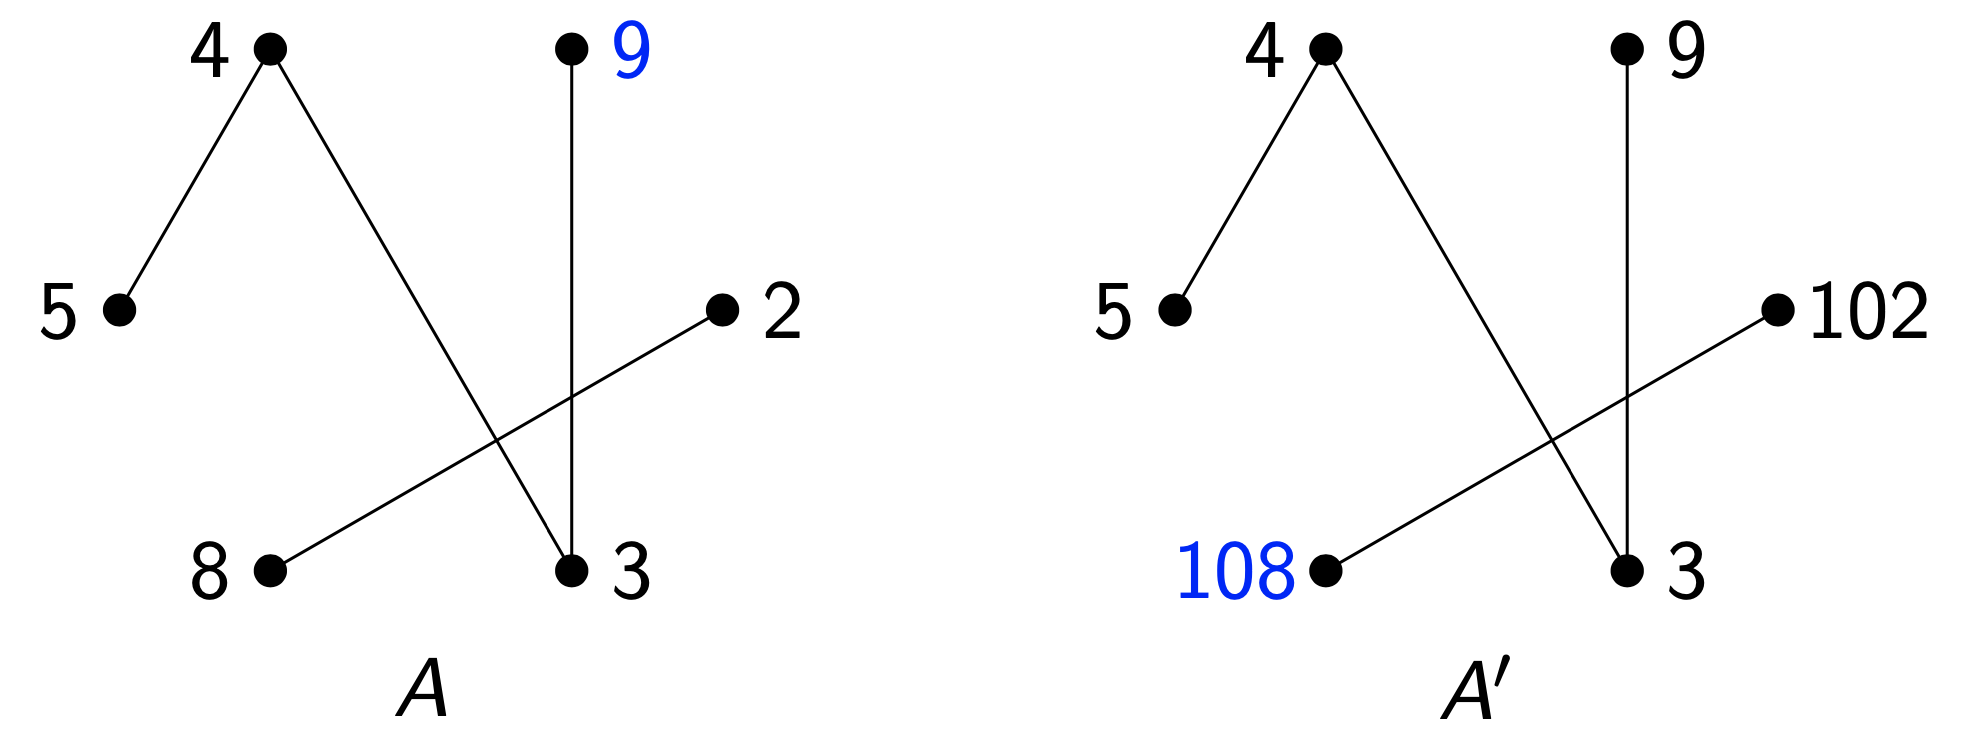
\includegraphics[width=0.7\linewidth]{maximum-problem-graph.png} 
        \item $M$ cannot differentiate $A$ and $A'$.
      \end{itemize}
    \item \definition{adversary argument} inputs are decided such that they have different solutions
  \end{itemize}

  \subsubsection{Second Largest Problem}
  \begin{itemize}
    \item \textit{problem}: find the second largest element in $<2n-3$ comparisons (2x Maximum $\Rightarrow$ $\scriptstyle (n-1) + ((n-1)-1) = 2n-3$ )
    \item \textit{solution}: \textbf{knockout tournament} $\Rightarrow n + \lceil \lg n \rceil - 2$
      \\* 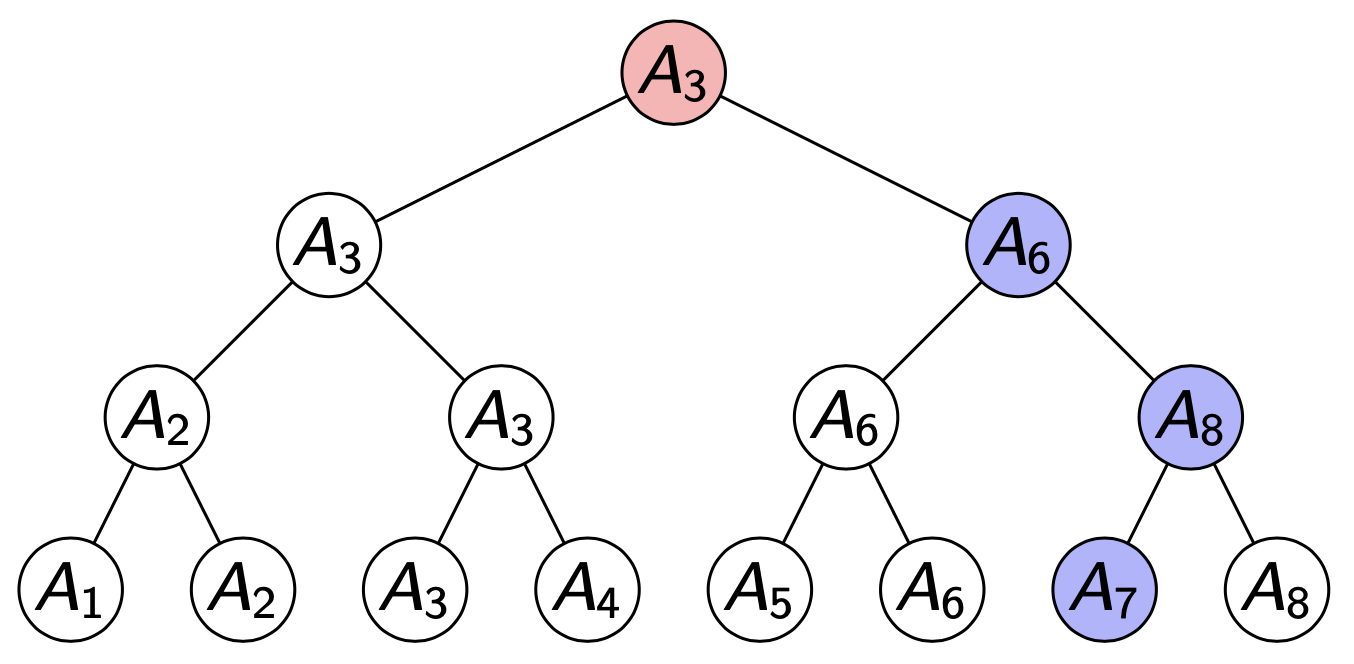
\includegraphics[width=0.6\linewidth]{second-largest-solution.png} 
      \begin{enumerate}
        \item bracket system: $n-1$ matches 
          \begin{itemize}
            \item every non-winner has lost exactly once
          \end{itemize}
        \item then compare the elements that have lost to the largest
          \begin{itemize}
            \item the second-largest element must have lost to the winner
            \item compares $\lceil \lg n \rceil$ elements that have lost to the winner using $\lceil \lg n \rceil -1$ comparisons 
          \end{itemize}
      \end{enumerate}
  \end{itemize}

  \subsubsection{Sorting}
  \begin{itemize}
    \item there is a sorting algorithm that requires $\leq n \lg n - n + 1$ comparisons.
    \item \textit{proof:} every sorting algorithm must make $\geq \lg (n!)$ comparisons.
      \begin{enumerate}
        \item let set $\mathcal{U}$ be the set of all permutations of the set $\{1, \dots, n\}$ that the adversary could choose as array $A$. $\vert \mathcal{U} \vert = n!$ 
        \item for each query "is $A_i > A_j$?", 
          \\* if $\mathcal{U}_{yes} = \{A \in \mathcal{U} : A_i > A_j\}$ is of size $\geq \vert\mathcal{U}\vert /2$, set $\mathcal{U} := \mathcal{U}_{yes}$. else: $\mathcal{U} := \mathcal{U} \backslash \mathcal{U}_{yes}$
        \item the size of $\mathcal{U}$ decreases by at most half with each comparison
        \item for $> \lg (n!)$ comparisons, $\mathcal{U}$ will still contain at least 2 permutations
      \end{enumerate}
  \end{itemize}

  \begin{tightcenter}
    $n! \geq (\frac{n}{e})^n$ 
    \\* $\Rightarrow \lg (n!) \geq n \lg (\frac{n}{e}) = n \lg n - n \lg e$
    \\* $\approx n \lg n - 1.44n$
    \\* $\Rightarrow$ roughly $n \lg n$ comparisons are \textbf{required} and \textbf{sufficient} for sorting $n$ numbers
  \end{tightcenter}

  \subsection{String Model}
  \begin{itemize}
    \item input: string of $n$ bits
    \item each query: find out \textbf{one bit} of the string
    \item $n$ queries are \textbf{necessary} and \textbf{sufficient} to check if the input string is all 0s.
  \end{itemize}

  \subsection{Graph Model}
  \begin{itemize}
    \item input: (symmetric) adjacency matrix of an $n$-node undirected graph
    \item each query: find out if an edge is present between two chosen nodes
    \item \textit{proof}: $\binom{n}{2}$ queries are necessary to decide whether the graph is connected or not
      \begin{enumerate}
        \item suppose $M$ is an algorithm making $\leq \binom{n}{2}$ queries.
        \item whenever $M$ makes a query, the algorithm tries not adding this edge, but adding all remaining unqueried edges. 
          \begin{enumerate}
            \item if the resulting graph is connected, $M$ replies $0$ (i.e. edge does not exist)
            \item else: replies $1$ (edge exists)
          \end{enumerate}
        \item after $< \binom{n}{2}$ queries, at least one entry of the adjacency matrix is unqueried.
      \end{enumerate}
  \end{itemize}


  \section{02. ASYMPTOTIC ANALYSIS}

  \begin{itemize}
    \item \definition{algorithm} a \textit{finite} sequence of well-defined instructions to solve a given computational problem
    \item \definition{runtime} measured in number of instructions taken in \textbf{word-RAM} model
      \begin{itemize}
        \item operators, comparisons, if, return, etc
      \end{itemize}
  \end{itemize}

  \subsection{Asymptotic Notations}

  \begin{tightcenter}
    \textbf{upper bound ($\leq$)}: $f(n) = O(g(n))$ 
    \\* if $\exists c>0, n_0>0$ such that $\forall n \geq n_0$, $\quad 0 \leq f(n) \leq cg(n)$ 
  \end{tightcenter}

  \begin{tightcenter}
    \textbf{lower bound ($\geq$)}: $f(n) = \Omega(g(n))$ 
    \\* if $\exists c>0, n_0>0$ such that $\forall n \geq n_0$, $\quad 0 \leq cg(n) \leq f(n)$ 
  \end{tightcenter}

  \begin{tightcenter}
    \textbf{tight bound}: $f(n) = \Theta(g(n))$ 
    \\* if $\exists c_1>0, c_2>0, n_0>0$ such that $\forall n \geq n_0, \quad 0 \leq c_1 g(n) \leq f(n) \leq c_2 g(n)$ 
  \end{tightcenter}

  \begin{tightcenter}
    \textbf{$o$ notation ($<$)}: $f(n) = o(g(n))$ 
    \\* if $\exists c>0, n_0>0$ such that $\forall n \geq n_0$, $\quad 0 \leq f(n) < cg(n)$ 
  \end{tightcenter}

  \begin{tightcenter}
    \textbf{$\omega$-notation ($>$)}: $f(n) = \omega(g(n))$ 
    \\* if $\exists c>0, n_0>0$ such that $\forall n \geq n_0$, $\quad 0 \leq cg(n) < f(n)$ 
  \end{tightcenter}

  \subsubsection{Set definitions}

  \begin{itemize}
    \item \textit{upper}: $O(g(n)) = $
      \\* $ \{f(n): \exists c>0, n_0>0 \mid \forall n \geq n_0, \, 0 \leq f(n) \leq cg(n)\}$
    \item \textit{lower}: $\Omega(g(n)) = $
      \\* $ \{f(n): \exists c>0, n_0>0 \mid \forall n \geq n_0, \, 0 \leq cg(n) \leq f(n)\}$
  \end{itemize}

  \begin{niceproof}
    that $2n^2 = O(n^3)$ 
    \\* let $f(n) = 2n^2$. then $f(n) = 2n^2 \leq n^3$ when $n \geq 2$. 
    \\* set  $c=1$ and $n_0 = 2$.
    \\* we have $f(n) = 2n^2 \leq c \cdot n^3$ for $n \geq n_0$. \qed
  \end{niceproof}

  \subsection{Limits}

  Assume $f(n), g(n) > 0$.
  \begin{center}
    $\lim\limits_{n \to \infty} \frac{f(n)}{g(n)} = 0 \Rightarrow f(n) = o(g(n))$
    \\* $\lim\limits_{n \to \infty} \frac{f(n)}{g(n)} < \infty \Rightarrow f(n) = O(g(n))$
    \\* $0 < \lim\limits_{n \to \infty} \frac{f(n)}{g(n)} < \infty \Rightarrow f(n) = \Theta(g(n))$
    \\* $\lim\limits_{n \to \infty} \frac{f(n)}{g(n)} > 0 \Rightarrow f(n) = \Omega(g(n))$
    \\* $\lim\limits_{n \to \infty} \frac{f(n)}{g(n)} = \infty \Rightarrow f(n) = \omega(g(n))$
  \end{center}

  \begin{niceproof}
    using delta epsilon definition
  \end{niceproof}

  \subsection{Properties of Big O}

  \begin{fixedbox}
    $\Theta(g(n)) = O(g(n)) \cap \Omega(g(n))$
  \end{fixedbox}

  \begin{itemize}
    \item $\textbf{transitivity}$ - applies for $O, \Theta, \Omega, o, \omega$
      $f(n) = O(g(n)) \land g(n) = O(h(n)) \Rightarrow f(n) = O(h(n))$ 
    \item \textbf{reflexivity} - for $O, \Omega, \Theta, \quad f(n) = O(f(n))$ 
    \item \textbf{symmetry} - $f(n) = \Theta(g(n)) \iff g(n) = \Theta(f(n))$
    \item \textbf{complementarity} - 
      \begin{itemize}
        \item $f(n) = O(g(n)) \iff g(n) = \Omega(f(n))$
        \item $f(n) = o(g(n)) \iff g(n) = \omega(f(n))$
      \end{itemize}
  \end{itemize}

  insertion sort: $O(n^2)$ with worst case $\Theta(n^2)$

  \begin{fixedbox}[0.8]
    $\log\log n < \log n < (\log n)^k < n^k < k^n$
  \end{fixedbox}























\end{multicols*}

\end{document}
